\newpage
\chapter{SYSTEM DESIGN}
% \begin{center}
%     \textbf{\LARGE SYSTEM DESIGN}\\[1cm]
% \end{center}

\justify
\section{System Architecture Overview} % (fold)

\begin{figure}[h!]
    \centering
    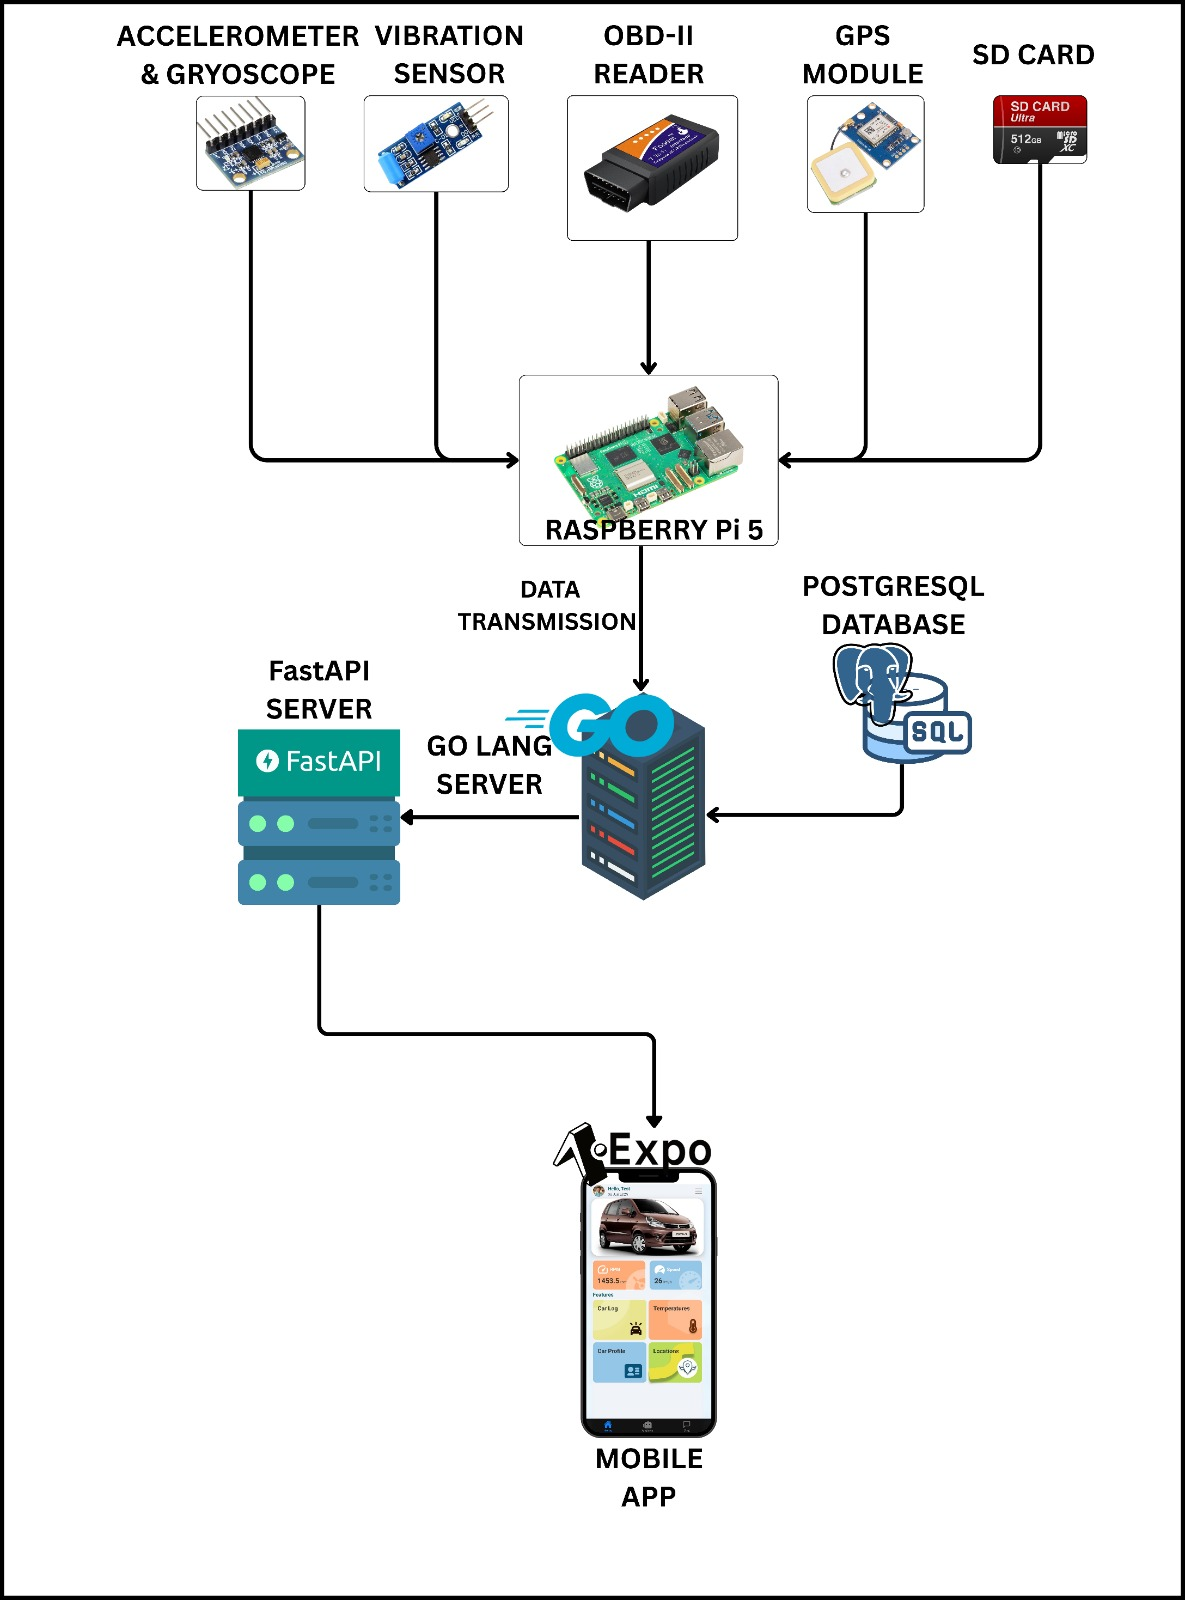
\includegraphics[width=0.8\textwidth]{assets/system_design_v2.jpeg}
    \caption{System Design Overview}
\end{figure}

The proposed vehicle diagnostic system integrates various components of hardware and software to collect real-time data for analysis. The architecture is designed to collect vehicle information via the OBD-II port, transmit it wirelessly to a cloud server for processing, and provide a visual representation of processed data through a mobile application. 
The system consists of 4 primary components: Hardware Implementation, Data processing using machine learning models, Servers and Databases, and a cross-platform mobile application. A block diagram representing the overall system architecture and data flow from vehicle sensors to end user presentation is shown in Figure 1.1


The diagram illustrates the flow of data and interactions within an automotive diagnostic and monitoring system. The system integrates multiple sensors, data processing units, databases, and APIs to achieve real-time diagnostics and data sharing. Below is a detailed explanation of the components and their interactions:

% \begin{enumerate}
%     \item \textbf{Sensor and Hardware Layer} At the core of the system lies the Raspberry Pi 5, which functions as the primary edge computing device. It interfaces with multiple onboard sensors and modules, including:
%         \begin{enumerate}
%             \item \textbf{Accelerometer & Gyroscope:} Captures motion dynamics and orientation data, essential for detecting aggressive maneuvers, collisions, or rollovers.
%             \item \textbf{Vibration Sensor:} Monitors abnormal vibrations indicative of impacts or mechanical faults.
%             \item \textbf{OBD-II Reader:} Establishes communication with the vehicle's ECU using standard automotive protocols (CAN, ISO 9141, KWP2000). It extracts critical diagnostic parameters such as RPM, throttle position, engine temperature, and fault codes.
%             \item \textbf{GPS Module:} Provides accurate geolocation and route data, enabling context-aware analytics such as incident mapping and route reconstruction.
%             \item \textbf{SD Card:} Facilitates local and persistent data storage, ensuring continuous logging even during network outages or vehicle downtimes.
%         \end{enumerate}
%     \item \textbf{Edge Device – Raspberry Pi 5} The Raspberry Pi 5 acts as the central processing unit at the vehicle level. It aggregates sensor inputs, performs real-time data processing, and securely transmits relevant information to the cloud server.
%     \item \textbf{API Interface – Golang server} The FastAPI Server hosts the core application logic. It does the Machine learning analysis of collected data. This includes analyzing driving behavior, detecting anomalies, and performing predictive diagnostics using pre-trained models. By handling these computations at the API level, the system ensures near real-time insights and intelligent decision-making at the edge.Its use of a performant and scalable language like Go ensures low-latency operations and robust backend performance.
%     \item \textbf{Database Layer – PostgreSQL} The PostgreSQL Database is the central repository for all collected and processed data. It maintains structured records of:
%     \item \textbf{User Interface – Mobile Application (Expo Framework):}
%     % image
%     \begin{figure}[h!]
%         \centering
%         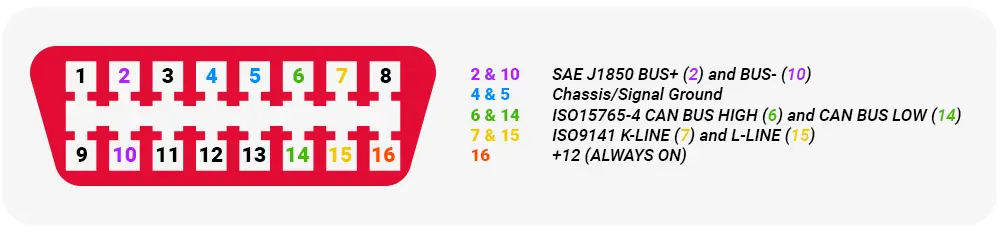
\includegraphics[width=13cm]{assets/obd_pinout.png}
%         \caption{OBD-II Connector Pin-out}
%         \label{fig:obd_pinout}
%     \end{figure}

%     The OBD-II standard specifies a 16-pin connector known as the J1962 connector, which is used universally across most vehicles. The pinout for this connector is defined as follows:

% \begin{table}[h!]
%     \centering
%     \caption{OBD-II Connector Pinout}
%     \label{table:obd_pinout}
%     \renewcommand{\arraystretch}{2.5} % Adjust row height (1 cm approx. with default font size)
%     \begin{tabular}{|c|l|}
%     \hline
%     \textbf{Pin} & \textbf{Function} \\ \hline
%     1  & Manufacturer discretion \\ \hline
%     2  & Bus positive Line (SAE J1850 PWM and VPW) \\ \hline
%     3  & Manufacturer discretion \\ \hline
%     4  & Chassis ground \\ \hline
%     5  & Signal ground \\ \hline
%     6  & CAN high (ISO 15765-4 and SAE J2284) \\ \hline
%     7  & K-line (ISO 9141-2 and ISO 14230-4) \\ \hline
%     8  & Manufacturer discretion \\ \hline
%     9  & Manufacturer discretion \\ \hline
%     10 & Bus negative Line (SAE J1850 PWM only) \\ \hline
%     11 & Manufacturer discretion \\ \hline
%     12 & Manufacturer discretion \\ \hline
%     13 & Manufacturer discretion \\ \hline
%     14 & CAN low (ISO 15765-4 and SAE J2284) \\ \hline
%     15 & L-line (ISO 9141-2 and ISO 14230-4) \\ \hline
%     16 & Battery voltage (+12 Volt for type A connector, +24 Volt for type B connector) \\ \hline
%     \end{tabular}
%     \end{table}
    




% The assignment of unspecified pins is left to the vehicle manufacturer's discretion, allowing for variations in implementation across different brands and models.

% The communication between the OBD system and the Engine Control Unit (ECU) occurs through standardized protocols. This communication involves several key components:

% Data Link Connector: The OBD-II connector serves as a physical interface for diagnostic tools to communicate with the ECU.
% Protocols: Various communication protocols are utilized, including:


% \begin{itemize}
%     \item ISO 9141-2
%     \item ISO 14230-4 (Keyword Protocol 2000)
%     \item ISO 15765-4 (CAN bus)
% \end{itemize}

% Parameter Identification (PID): PIDs are specific data points that can be queried from the ECU. They provide information about various vehicle parameters such as engine RPM, vehicle speed, coolant temperature, etc. Each PID corresponds to a specific function or piece of data that the ECU can report back to diagnostic tools.

% \item \textbf{Python Script} A Python script retrieves data from the ECU and processes it for further analysis or storage. It acts as a bridge between the raw sensor data and the database/server layer.

% \item \textbf{Postgres Database} The Postgres database serves as the primary storage for processed telemetry data. It provides a structured and reliable backend for managing sensor data and results from further computations.

% \item \textbf{Go Server} The Go server processes data stored in the Postgres database and performs additional tasks, such as:
% \begin{itemize}
%     \item Data aggregation
%     \item Complex computations or analytics
%     \item API responses for connected systems
% \end{itemize}
% \item \textbf{FastAPI Script} The FastAPI script interacts with the Postgres database to:
% \begin{itemize}
%     \item Expose APIs for retrieving or upserting data
%     \item Enable data queries from other applications or systems
%     \item Provide endpoints for monitoring, diagnostics, and reporting
% \end{itemize}
% \newpage
% \item \textbf{Mobile App} The app provides the user interface for interacting with the system. Through the integration with a Golang server and PostgreSQL database, the app can:
% \begin{itemize}
%     \item Display real-time telemetry data
%     \item Provide diagnostic reports
%     \item Enable user interaction and configuration of the system
% \end{itemize}
% \end{enumerate}
